\section{Simulations}

\subsection{Constant heat source and thermal conductivity}
\label{sec:simu_constant}

The first set of simulations will be done considering an ideal case, as in \autoref{sec:solution_anal}. The heat source was chosen to be \(S(r) \equiv S_0 = 1000\) \si{\watt\per\cubic\meter} and the conductivity of the cylinder \(\kappa(r) \equiv \kappa_0 = 10^{-3}\) \si{\watt\per\meter\per\kelvin}. Taking \(\sigma = 10^{10}\) enlarges the spreak of \(\kappa\), allowing us to consider it constant between \(r=0\) and \(r=R\).

Using a small amount of mesh intervals (\(N=10\)), the temperature and heat flux were obtained, as shown in \autoref{fig:temperature_constant} and \autoref{fig:heat_constant} respectively. The analytical solution is plotted alongside the simulation data. We can see that the temperature gradient is higher at the edge of the cylinder than close to its center, as expected. The heat flux also remains very linear with respect to \(r\), except when close to the center. This will be discussed later. Close to the border of the cylinder (\(r=R\)), the simulations match the analytical solution quite closely. Closer to the center however, the uniform (equidistant in \(r\)) mesh remains a lot closer to the analytical solution, while the non-uniform mesh (equidistant in \(r^2\)) seems to become linear. This could be explained by the sparcity of mesh nodes close to the center, the first one being at \(r=0\) \si{\centi\meter} and the second one at \(r \approx 1.5\) \si{\centi\meter}, alongside the piecewise linear interpolating functions \(\Lambda_i\). A similar phenomenon can be seen in the heat flux, where the heat flux was calculated at the center of each interval.

\begin{figure}[h]
    \centering
    \begin{subfigure}{0.5\linewidth}
        \centering
        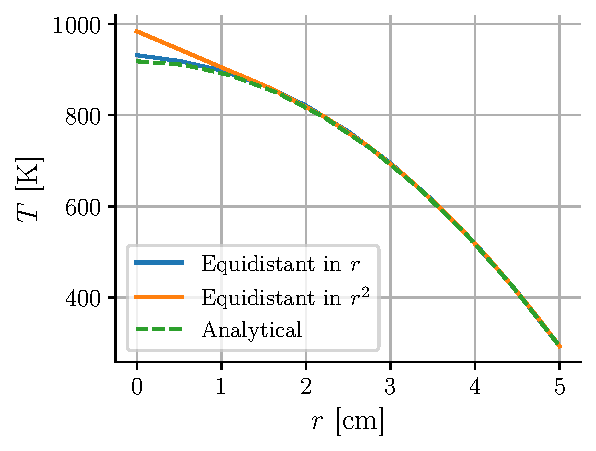
\includegraphics[width=\linewidth]{figures/temperature_constant.pdf}
        \caption{Temperature}
        \label{fig:temperature_constant}
    \end{subfigure}
    \begin{subfigure}{0.48\linewidth}
        \centering
        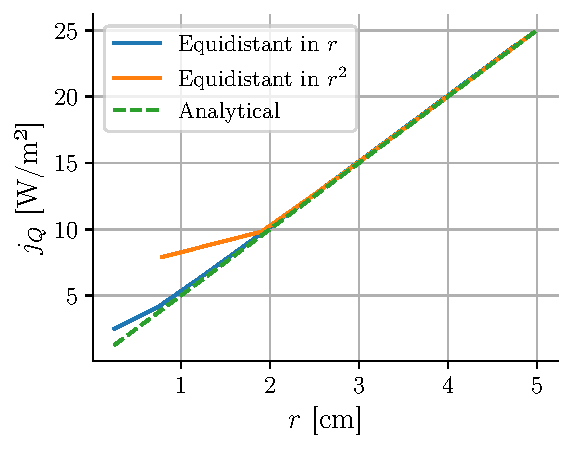
\includegraphics[width=\linewidth]{figures/heat_constant.pdf}
        \caption{Heat flux}
        \label{fig:heat_constant}
    \end{subfigure}
    \caption{Temperature and heat flux for \(N = 10\) mesh intervals, constant heat source \(S_0 = 1000\) \si{\watt\per\meter\cubed} and constant thermal conductivity \(\kappa = 10^{-3}\) \si{\watt\per\meter\per\kelvin}}
\end{figure}

The total power of the cylinder is given by \(\int_{0}^{R} S(r) 2\pi r \dd r = S_0 \pi R^2\) \si{\watt}, which should in theory be equal to the heat flux at the cylinder's border \(\Gamma_Q(R) = 2 \pi R j_Q(R)\) \si{\watt}. Using the heat flux computed inside the simulation closest to the border (\(r=R\)), the error on the global power balance is reported in \autoref{tab:error_global_power_constant}. One explanation for the difference comes from where the heat flux was measured: at the center of the final interval. Adjusting the total power to be calculated for \(r\) at the midpoint of the final interval yields much better results, lowering the relative deviation to 0.2\% for the uniform mesh and 0.06\% for the non-uniform mesh. It does then seem reasonable to assume that the global power balance is satisfied. The greater accuracy of the non-uniform mesh probably stems from the fact that the final midpoint is closer to \(R\) than the final midpoint of the uniform mesh.

\begin{table}[h]
    \centering
    \begin{tabulary}{\linewidth}{C|C C C C}
        \toprule
        & \(P_\textrm{tot}\) [\si{\watt}] & \(\Gamma_Q(R)\) [\si{\watt}] & Difference to \(P_\textrm{tot}(R)\) [\si{\watt}] & Relative deviation [\%] \\
        \midrule
        Uniform & 7.85 & 7.11 & 0.75 & 9.5 \% \\
        Non-uniform & 7.85 & 7.46 & 0.39 & 5.0 \% \\
        \bottomrule
    \end{tabulary}
    \caption{Error on global power balance for uniform and non-uniform mesh}
    \label{tab:error_global_power_constant}
\end{table}

Let's analyse the convergence of the finite element method under this system. Firstly, the error with respect to the analytical solution on the temperature at the center of the cylinder \(T(0)\) as a function of \(\frac{1}{N}\), where \(N\) is the number of mesh intervals, is shown in \autoref{fig:convergence_temp_N_constant}. We can see that the uniform mesh converges in order 2 while the non-uniform mesh converges in order 1. It is interesting to note that the actual order of convergence for the uniform mesh is 1.84, which we will consider to be order 2. The same error was also plotted as a function of the largest interval size in \autoref{fig:convergence_temp_interval_constant}. In this case, both mesh configurations converge in order 2. Again, the uniform mesh is closer to an order of 1.84, meaning that the temperature at the center converges faster with respect to the bigest interval size in the non-uniform case than the uniform case. For the same biggest interval size, the error with the non-uniform mesh is a bit smaller than the uniform mesh.

\begin{figure}[h]
    \centering
    \begin{subfigure}{0.48\linewidth}
        \centering
        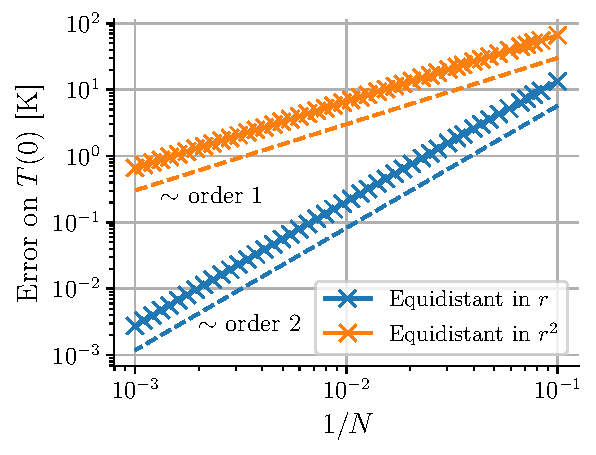
\includegraphics[width=\linewidth]{figures/convergence_temp_N_constant.pdf}
        \caption{Depending on mesh resolution}
        \label{fig:convergence_temp_N_constant}
    \end{subfigure}
    \begin{subfigure}{0.48\linewidth}
        \centering
        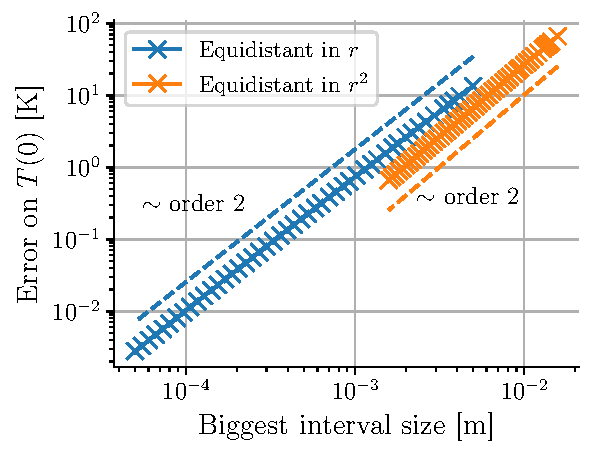
\includegraphics[width=\linewidth]{figures/convergence_temp_interval_constant.pdf}
        \caption{Depending on maximum interval length}
        \label{fig:convergence_temp_interval_constant}
    \end{subfigure}
    \caption{Convergence of temperature at the center of the cylinder, with constant heat source \(S_0 = 1000\) \si{\watt\per\meter\cubed} and constant thermal conductivity \(\kappa = 10^{-3}\) \si{\watt\per\meter\per\kelvin}}
    \label{fig:convergence_temp_constant}
\end{figure}

The convergence of the heat flux at the border of the cylinder \(j_Q(R)\) was also studied. \autoref{fig:convergence_heat_constant} shows that both mesh layouts converge with exactly order 1. The error with respect to the analytical solution is a bit lower for the non-uniform mesh than the uniform mesh. This could be explained by the higher point density close to \(R\) of the non-uniform mesh, yielding a better approximation of the temperature gradient close to \(R\). Similarly to the convergence of the heat flux at the border, the error on the global power balance decreases with order 1 with respect to \(\frac{1}{N}\), as shown in \autoref{fig:error_power_balance_constant}. The minimal error obtained here was for \(N = 1000\), which gave an error on the order of \(10^{-3}\), which isn't great but also not terrible. This means that for a very accurate simulation, if we want to conserve the global power balance, we would need a very fine mesh.

\begin{figure}[h]
    \begin{minipage}{0.47\linewidth}
        \centering
        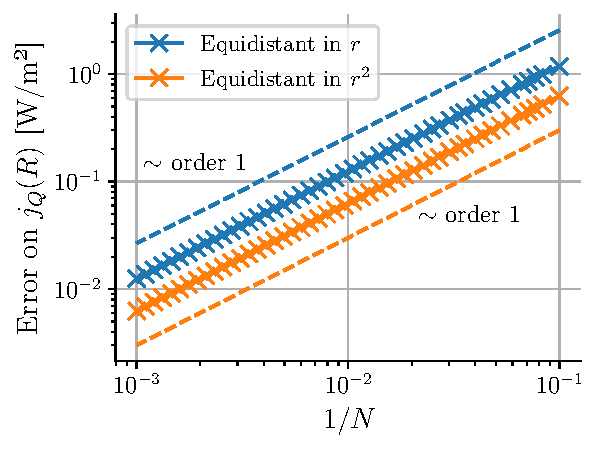
\includegraphics[width=\linewidth]{figures/convergence_heat_N_constant.pdf}
        \captionof{figure}{Convergence of heat flux at the cylinder's border \(r=R\), with constant heat source \(S_0 = 1000\) \si{\watt\per\meter\cubed} and constant thermal conductivity \(\kappa = 10^{-3}\) \si{\watt\per\meter\per\kelvin}}
        \label{fig:convergence_heat_constant}
    \end{minipage}
    \hspace{0.5cm}
    \begin{minipage}{0.5\linewidth}
        \centering
        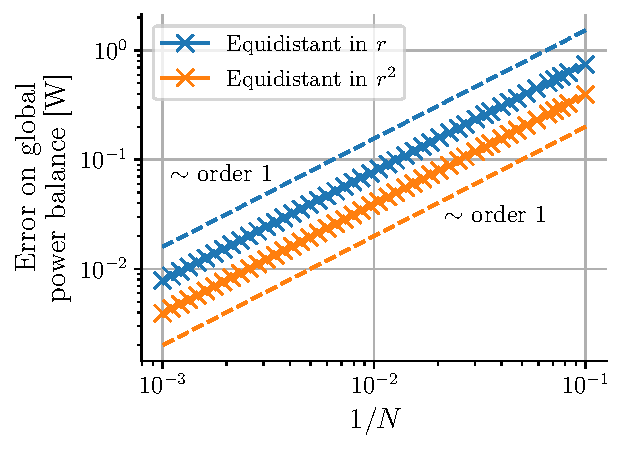
\includegraphics[width=\linewidth]{figures/convergence_power_balance_N_constant.pdf}
        \captionof{figure}{Error on global power balance \(|P_{\textrm{tot}} - \Gamma_Q(R)|\), with constant heat source \(S_0 = 1000\) \si{\watt\per\meter\cubed} and constant thermal conductivity \(\kappa = 10^{-3}\) \si{\watt\per\meter\per\kelvin}}
        \label{fig:error_power_balance_constant}
    \end{minipage}
\end{figure}

\subsection{Varying heat source and thermal conductivity}

...

\subsection{Changing integration method}

The integration method for initialising the matrix elements can also be changed. Until now, the midpoint rule was used. The implementation was changed to allow a mix of the trapezoidal rule and midpoint rule, with a parameter \(p\) setting the weight of each method. Setting \(p = 0\) means only using the midpoint rule and \(p = 1\) is only the trapezoidal rule. The formula for integration then becomes:
\begin{equation}
    \int_{x_k}^{x_{k+1}} f(x) \dd x \approx h_k \left[ p \frac{f(x_k) + f(x_{k+1})}{2} + (1-p) f \left( \frac{x_k + x_{k+1}}{2} \right) \right]
\end{equation}
Using the same configuration as in \autoref{sec:simu_constant}, we obtain a temperature and heat flux as shown in \autoref{fig:temperature_exact} and \autoref{fig:heat_exact}. A very interesting phenomenon occured: in both cases, the simulations match the analytical solution exactly at the mesh nodes, while only differing in between nodes due to the linear interpolation! This is because \textbf{FEUR MARTIN OSKOUR}.

\begin{figure}[h]
    \centering
    \begin{subfigure}{0.5\linewidth}
        \centering
        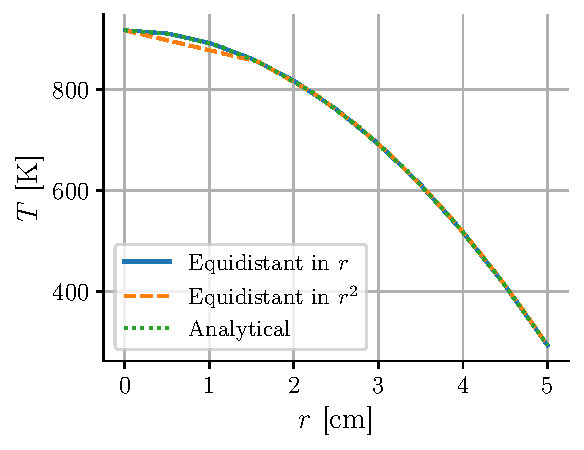
\includegraphics[width=\linewidth]{figures/temperature_exact.pdf}
        \caption{Temperature}
        \label{fig:temperature_exact}
    \end{subfigure}
    \begin{subfigure}{0.48\linewidth}
        \centering
        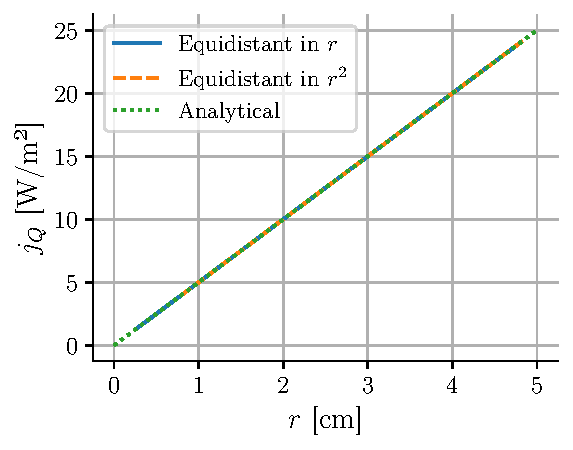
\includegraphics[width=\linewidth]{figures/heat_exact.pdf}
        \caption{Heat flux}
        \label{fig:heat_exact}
    \end{subfigure}
    \caption{Temperature and heat flux for \(N = 10\) mesh intervals, constant heat source \(S_0 = 1000\) \si{\watt\per\meter\cubed} and constant thermal conductivity \(\kappa = 10^{-3}\) \si{\watt\per\meter\per\kelvin}}
\end{figure}
